
Порождающие модели современное и быстро развивающие направление работы с данными.

Ключевыми достижениями в дисципилине были \begin{enumerate}
    \item порождающие грамматики \cite{chomsky2002syntactic}
    \item графические вероятностные модели \cite{pearl1988probabilistic}
    \item состязательные порождающие модели \cite{goodfellow2020generative}
    \item диффузионные порождающие модели \cite{song2020score}
\end{enumerate}

Порождающие модели задают совместное распределение наблюдаемого объекта $x$ и его черт $y$ -  $p(x,y)$. В этом заключается 
ключевое различие между порождающими и дискриминирующими моделями $p(y|x)$ \ref{discr_vs_gen}.

\begin{figure}[h]
    \centering
    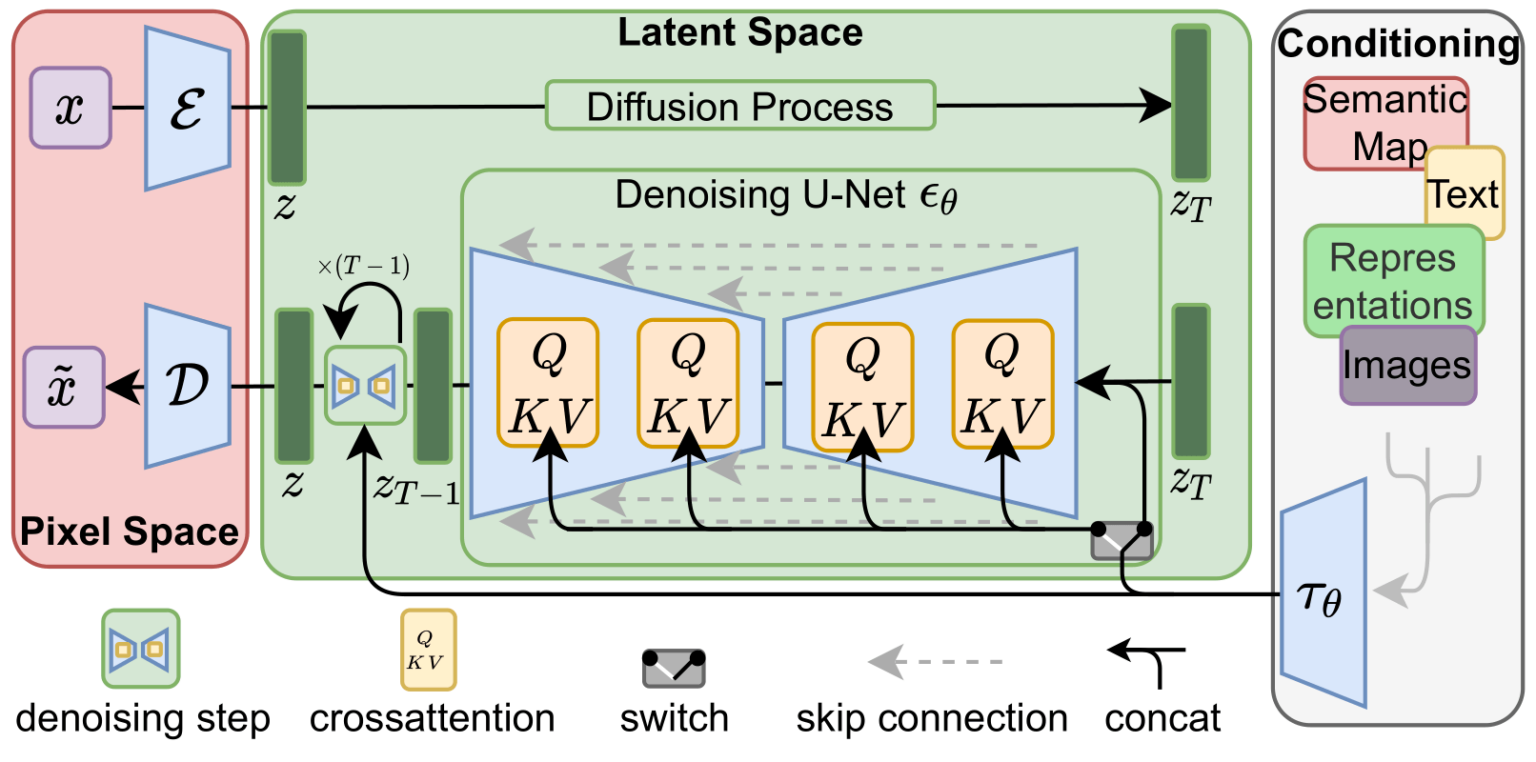
\includegraphics[width=0.5\textwidth]{assets/ml/generation/stable_diffusion.png}
    \caption{Генеративные отличаются}
    \label{discr_vs_gen}
\end{figure}


Порождающие модели, используют параметрические модели $p_\theta$ для аппроксимации истинных функций распределений.
Таким образом,


Простейшим видом порождающей модели является авторегрессионую модель,
 использующую разложение вероятности через цепочку условных вероятностей для аппроксимации:
\begin{equation}
    p(\mathbf{x}) = p(x_1) p(x_2 |x_1) \dots p(x_n|x_1,\dots,\x_n)
\end{equation}

\textit{Определение } \textbf{Авторегрессионные модели} представляют собой класс порождающих моделей,
с вычислимой  вероятностью, выполняющие генерацию через цепочку последовательных преобразований \begin{equation}
    p(x^{(1)},\dots,x^{(t)}) = \prod_{t=1}^T p(x^{(t)}|x^{(1)},\dots,x^{(t-1)})
\end{equation}
Авторегрессионные модели могут быть реализованы с использованием различных подходов, 
включая марковские модели, рекуррентные нейронные сети и модели с авторегрессионными свойствами, такие как GPT (Generative Pre-trained Transformer) и LSTM (Long Short-Term Memory). 
Они находят применение в широком спектре задач обработки естественного языка, включая генерацию текста, машинный перевод, синтез речи и другие.

\begin{equation}
    \mathrm E_{p(\mathbf{x})} f(\mathbf{x}) = \int p(\mathbf{x}) f(\mathbf{x}) dx \approx \frac{1}{n} \sum_i=1^n f(x_i)
\end{equation}


\textit{Определение} $f$-дивергенцией называется выпуклая функция, удовлетворяющая равенству $f(1)=0$/

$$
    D_f{\pi \parallel \rho} = \mathrm E_{\rho(x)} f\left(\frac{\pi(x)}{\rho(x)}\right)
$$

Семейство $f$-дивергенций включает функции \begin{enumerate}
    \item Кульбака-Лейбнера $f(u)=u logu $
\end{enumerate}


\texit{Определение} \textbf{EM-алгоритм} - алгоритм для нахождения оценок
максимального правдоподобия параметров 
 вероятностных моделей с скрытыми переменными $\theta$.

Алгоритм состоит из двух шагов. \begin{itemize}
    \item E(xpectation) шага $q^{(t)} = $. Шаг 
    обновляет распределение при фиксированных параметрах
    \item M(maximization)
\end{itemize}

Таким образом параметра $\Theta$ является
{\displaystyle \Theta _{n+1}} — это значение, максимизирующее $M$ условное матожидание $E$ логарифма правдоподобия при данных значениях наблюдаемых переменных и предыдущем значении параметров. 


Неравенство Йенсена 

$$
$$

Вариационный вывод (ELBO)

$$
    \mathcal{L}(\theta)
$$

